\subsection{The need for parallelism}

Over the previous few decades, a trend of ever-increasing hardware clock-speeds has fuelled developer complacency.
The often-cited ``Moore's Law''~\cite{moores_law} suggested that our favourite algorithms will scale with demand, as executing systems increase in performance alongside complexity.

\begin{figure}[h]
  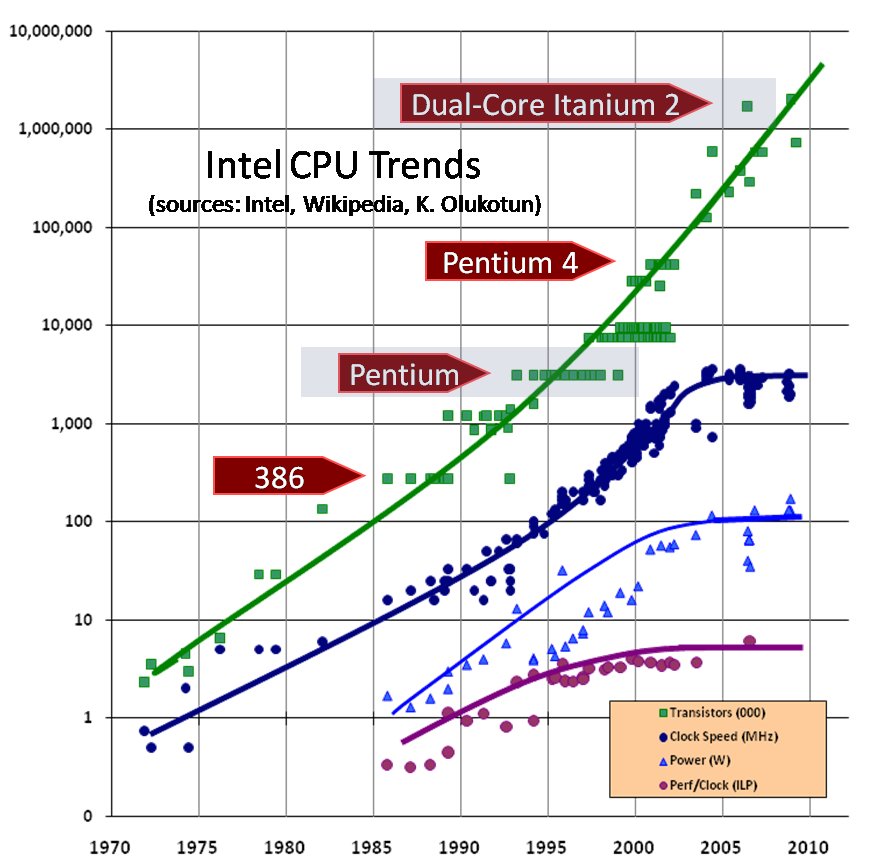
\includegraphics[width=0.8\textwidth]{./figures/free_lunch_over.png}
  \caption{Graph demonstrating the recent plateau in clock-speed increase and performance-per-clock. Source:~\cite{free_lunch_over}}
  \label{fig:free_lunch_over}
\end{figure}

The stark truth is that this trend now seems to have lapsed (Figure~\ref{fig:free_lunch_over}).
The latest generation of \acp{CPU} offer no significant clock-speed improvements over the previous. Furthermore, increases in per-clock performance are lacklustre.
Physical hardware constraints are to blame for this disappointment. Namely, higher-than-anticipated levels of interference between subcomponents as a result of vastly increased circuit densities.

To combat this stall, hardware manufacturers have responded by increasing the number of independent execution units, or \emph{cores}, present on produced system components. As a result, the total throughput available on any given class of device has continued to improve.
Today's data-driven economy generates computational problems of relentlessly increasing size. Therefore, software engineers must adapt to utilise this increased core-count.

Unfortunately, this tactic of improving performance, by presenting a greater number of compute-units, is often incompatible with traditional programming approaches. The inapplicability of many tried-and-tested sequential architectural patterns forces engineers to consider new ones.

Constructing a parallel solution requires the study of new concepts, such as synchronisation and data dependencies. The next generation of software engineers are becoming familiar with these issues, but there is currently a significant knowledge-gap.

The necessary switch to parallel programming is not going as smoothly as desired. A short term solution for easing this transition is to provide common developers with the capability to easily utilise all compute-units within a system.
